\section{Integration and Tool Support}\label{sec:integration}
%\ugh{A robust metamodel for traceability must be able to satisfy different needs and to that purpose shall be conceived in a modular way that allows potential users to take the parts of the metamodel they need in their scenario.}

An Xtext-based\footnote{\url{https://www.eclipse.org/Xtext/}} definition of our metamodel is available on a Git repository\footnote{\url{https://github.com/ebatot/TraceaDSL}}. As concrete syntax, we are using the JSON textual syntax shown in the examples above and illustrated in \Fig{fig:plugin}. 

\begin{figure}[ht] 
	\centering
	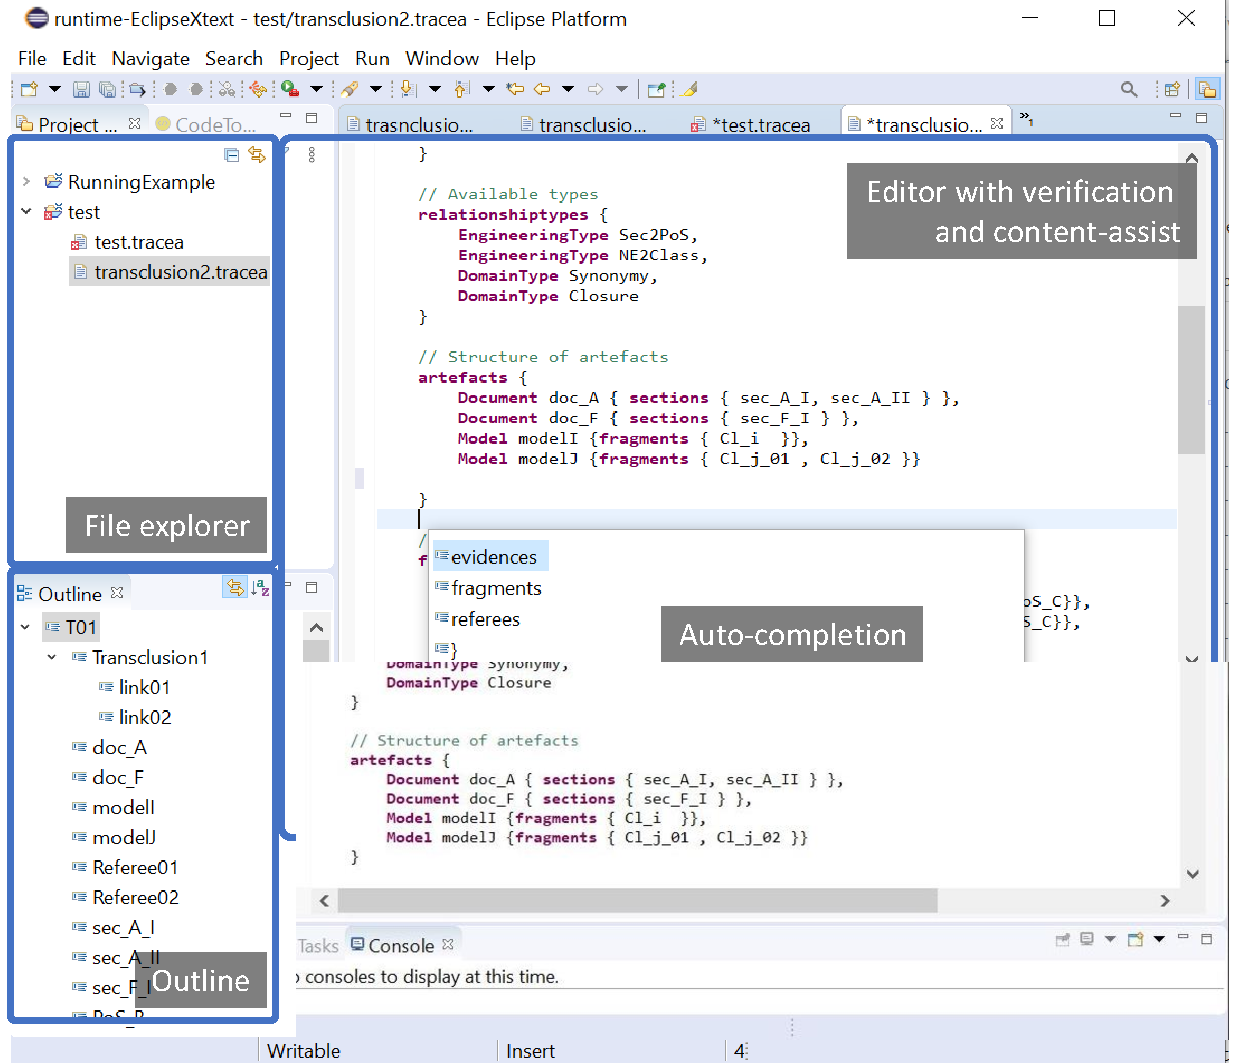
\includegraphics[width=.7\linewidth]{images/plugin-screenshot.pdf}
	\caption{Trace\textit{a} Xtext plugin}
	
	\label{fig:plugin}
\end{figure}


Beyond this option, we have also integrated Trace\textit{a} on top of Capra\footnote{\url{https://projects.eclipse.org/projects/modeling.capra}}. Eclipse Capra is a traceability management tool offering some interesting features to edit and visualize traces, including traceability matrices and graph visualisations. Capra includes a customization language based on Xcore\footnote{\url{https://wiki.eclipse.org/Xcore}}  we have used to add Trace\textit{a} concepts as Capra extensions. %. We employ this mechanism to integrate in the concept of trace link the quality aspects we defined earlier
Thanks to this integration you can benefit from the advanced metamodeling concepts in Trace\textit{a} while also enjoying Capra's visualization capabilities.  

In both cases, the designer can use Trace\textit{a} as a standalone tool or add it as a new component to any model-driven pipeline, especially implemented on top of the EMF Eclipse ecosystem. 

As, in complex scenarios, traces can come from different systems (using different languages or even third-party APIs), it is useful to keep Trace\textit{a} as an \textit{external language} that you can adapt to the changing needs of your application scenario and the types of artefacts you need to trace  \cite{clelandhuang2007bestPracticeForAutomatedTraceability,maro2016_maintenance_factors_and_guidelines}. 

But as a trade-off, this forces designers to learn and add to their toolset a new language. An alternative option is to define Trace\textit{a} as kind of internal DSL, embedded in a more general modeling language like SysML or UML using the extension capabilities offered by them, e.g. UML profiles. 
 
 %Yet, traceability techniques are gaining ground in the engineering of dedicated languages. \textit{E.g.,} IBM Rational DOORS and OMG SysML are built with interfaces for generic traceability -- it is \textit{embedded} in their specification. 

